\newpage
\section{分子动理论的平衡态理论}

\begin{question}{题目2.2.1}
    在下图中列出某量 $x$ 的值的三种不同概率分布函数的图线,试对于每一种图线求出常量 $A$ 的值,使在此值下该函数成为归一化函数. 然后计算 $x$ 和 $x^2$ 的平均值,在第一种情形下还应该求出 $|x|$ 平均值.
    \begin{center}

        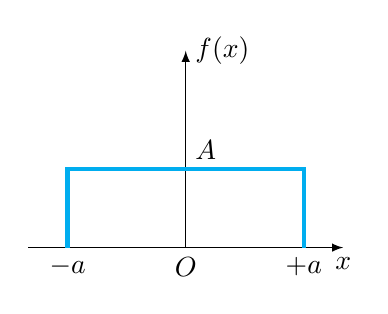
\begin{tikzpicture}
            \label{x的概率密度函数a}
            \draw[-latex] (-2, 0) -- (2, 0) node[below] {$x$};
            \draw[-latex] (0, 0) -- (0, 2.5) node[right] {$f(x)$};
            \node[below] (O) at (0,0) {$O$};

            \draw[ultra thick, cyan] (-1.5, 0) -- (-1.5, 1) -- (1.5, 1) -- (1.5, 0);

            \node[below] at (-1.5, 0) {$-a$};
            \node[below] at (1.5, 0) {$+a$};
            \node[above right] (A) at (0, 1) {$A$};
        \end{tikzpicture}
        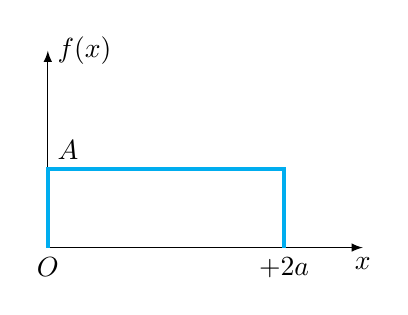
\begin{tikzpicture}
            \label{x的概率密度函数b}
            \draw[-latex] (0, 0) -- (4, 0) node[below] {$x$};
            \draw[-latex] (0, 0) -- (0, 2.5) node[right] {$f(x)$};
            \node[below] at (0,0) {$O$};

            \draw[ultra thick, cyan] (0, 0) -- (0, 1) -- (3, 1) -- (3, 0);

            \node[below] at (3, 0) {$+2a$};
            \node[above right] at (0, 1) {$A$};
        \end{tikzpicture}
        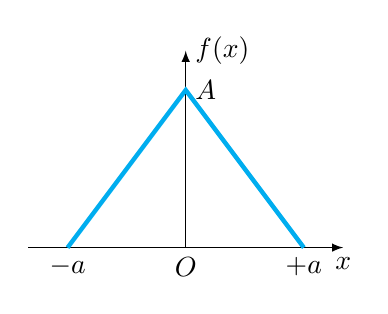
\begin{tikzpicture}
            \label{x的概率密度函数c}
            \draw[-latex] (-2,0) -- (2,0) node[below] {$x$};
            \draw[-latex] (0,0) -- (0,2.5) node[right] {$f(x)$};
            \node[below] at (0,0) {$O$};

            \draw[ultra thick, cyan] (-1.5, 0) -- (0, 2) -- (1.5, 0);

            \node[below] at (-1.5, 0) {$-a$};
            \node[below] at (1.5, 0) {$+a$};
            \node[right] at (0, 2) {$A$};
        \end{tikzpicture}
    \end{center}
\end{question}

\begin{solution}
    连续型随机变量的概率密度有如下性质:
    \begin{equation}
        \int_{-\infty}^{+\infty} f(x) \,\mathrm{d}x = 1
    \end{equation}
    \begin{equation}
        \overline{g(x)} = \int_{-\infty}^{+\infty} f(x)g(x) \,\mathrm{d}x
    \end{equation}

    \paragraph{对于(a)图} 按照归一化条件, 概率密度分布曲线下的面积为 $1$ ,则
    $$
        A = \frac{1}{2a}.
    $$
    $x$ 的概率密度为
    $$
        f(x) = \begin{dcases}
            \frac{1}{2a}, & -a \leqslant x \leqslant a, \\
            0,            & \text{其他}.
        \end{dcases}
    $$
    由此计算 $\overline{x}$ , $\overline{x^2}$ 和 $\overline{|x|}$
    $$
        \overline{x}
        = \int_{-a}^{+a} x f(x) \,\mathrm{d}x
        = \frac{1}{2a}\int_{-a}^{+a} x \,\mathrm{d}x
        = \frac{1}{2a}\left.\frac{x^2}{2}\right|_{-a}^{+a}
        = 0
    $$
    $$
        \overline{x^2}
        = \int_{-a}^{+a} x^2 f(x) \,\mathrm{d}x
        = \frac{1}{2a}\int_{-a}^{+a} x^2 \mathrm{d}x
        = \frac{1}{2a}\left.\frac{1}{3}x^3\right|_{-a}^{+a}
        = \frac{a^2}{3}
    $$
    $$
        \overline{|x|}
        = \int_{-a}^{0} -x f(x) \,\mathrm{d}x + \int_{0}^{a} x f(x) \,\mathrm{d}x
        = \int_{-a}^0 -\frac{1}{2a}x\,\mathrm{d}x + \int_0^a \frac{1}{2a}x\,\mathrm{d}x
        = \frac{a}{2}
    $$

    \paragraph{对于(b)图} 按照归一化条件,概率密度分布曲线下的面积为 $1$ ,则
    $$
        A = \frac{1}{2a}
    $$
    $x$ 的概率密度为
    $$
        f(x) = \begin{dcases}
            \frac{1}{2a}, & 0 \leqslant x \leqslant 2a, \\
            0,            & \text{其他}.                  \\
        \end{dcases}
    $$
    由此计算 $\overline{x}$ 和 $\overline{x^2}$
    $$
        \overline{x}
        = \int_{0}^{2a} x f(x) \,\mathrm{d}x
        = \frac{1}{2a}\int_{0}^{2a} x \,\mathrm{d}x
        = \left.\frac{1}{2a} \frac{x^2}{2}\right|_{0}^{2a}
        = a
    $$
    $$
        \overline{x^2}
        = \int_{0}^{2a} x^2 f(x) \,\mathrm{d}x
        = \frac{1}{2a}\int_{0}^{2a} x^2 \mathrm{d}x
        = \frac{1}{2a} \left.\frac{x^3}{3}\right|_{0}^{2a}
        = \frac{4a^2}{3}
    $$

    \paragraph{对于(c)图} 按照归一化条件,概率密度分布曲线下的面积为 $1$,则
    $$
        A = \frac{1}{a}.
    $$
    $x$ 的概率密度为
    $$
        f(x) = \begin{dcases}
            \frac{1}{a^2}x + \frac{1}{a},  & -a \leqslant x < 0, \\
            -\frac{1}{a^2}x + \frac{1}{a}, & 0 < x \leqslant a,  \\
            0,                             & \text{其他}.          \\
        \end{dcases}
    $$
    由此计算 $\overline{x}$ 和 $\overline{x^2}$
    $$
        \overline{x}
        = \int_{-a}^{+a} x f(x) \,\mathrm{d}x
        = \int_{-a}^{0} \left(\frac{1}{a^2}x^2 + \frac{1}{a}x\right) \mathrm{d}x +  \int_{0}^{a} \left(-\frac{1}{a^2}x^2 + \frac{1}{a}x\right) \mathrm{d}x
        = 0
    $$
    $$
        \overline{x^2}
        = \int_{-a}^{+a} x^2 f(x) \,\mathrm{d}x
        = 2\int_0^a \left(-\frac{1}{a^2}x^3 + \frac{1}{a}x^2 \right) \mathrm{d}x
        =  2\left.\left(-\frac{1}{4a^2}x^4 + \frac{1}{3a}x^3 \right)\right|_0^a = \frac{a^2}{6}
    $$
\end{solution}

\begin{question}{题目2.3.2}
    求速率在区间 $v_p \to 1.01v_p$ 内的气体分子数占总分子数的比率.
\end{question}
\begin{solution}
    麦克斯韦速率分布为
    \begin{equation}
        \frac{\mathrm{d}N}{N} = f(v) \,\mathrm{d}v = 4\pi\left(\frac{m}{2\pi kT}\right)^{3/2} \cdot \exp\left(-\frac{mv^2}{2kT}\right) \cdot v^2 \, \mathrm{d}v
    \end{equation}
    考虑到题目设定的速率区间与 $v_p$ 有关,故考虑用 $v_p = \sqrt{\dfrac{2kT}{m}}$ 改写上式
    $$
        \frac{\mathrm{d}N}{N} = f(v) \,\mathrm{d}v
        = \frac{4}{\sqrt{\pi}}\left(\frac{1}{v_p^2}\right)^{3/2} \cdot \exp\left(-\frac{v^2}{v_p^2}\right) \cdot v^2 \,\mathrm{d}v
    $$
    虽然因式 $\exp\left(-\dfrac{v^2}{v_p^2}\right)$ 很难直接处理,但是我们可以考虑用 $u = \dfrac{v}{v_p}$ 换元,进一步得到
    $$
        \frac{\mathrm{d}N_u}{N} = \frac{4}{\sqrt{\pi}}\left(\frac{1}{v_p^2}\right)^{3/2} \cdot \exp(-u^2) \cdot (uv_p)^2 \,\mathrm{d}(uv_p)  = \frac{4}{\sqrt{\pi}}\cdot\exp(-u^2)\cdot u^2 \,\mathrm{d}u
    $$
    相应地, 速率区间 $v_p \leqslant v \leqslant 1.01v_p$ 也会随着换元而变为 $1 \leqslant u \leqslant 1.01$. 注意到这是一个非常非常窄的区间,所以可以近似认为 $u = 1$, $\mathrm{d}u = 0.01$
    $$
        \frac{\mathrm{d}N_u}{N}
        \approx \frac{4}{\sqrt{\pi}} \cdot \mathrm{e}^{-1} \cdot 1^2 \cdot 0.01
        \approx 0.83\%.
    $$
\end{solution}

\begin{question}{题目2.3.4}
    根据麦克斯韦速率分布,求速率倒数的平均值 $\overline{\left(\dfrac{1}{v}\right)}$
\end{question}

\begin{solution}
    $$
        \begin{aligned}
            \overline{\left(\dfrac{1}{v}\right)}
             & = \int_0^{+\infty} \frac{1}{v} \cdot 4\pi \left(\frac{m}{2\pi kT}\right)^{3/2} \cdot \exp\left(-\frac{mv^2}{2kT}\right) \cdot v^2 \,\mathrm{d}v \\
             & = \int_0^{+\infty} \frac{4}{\sqrt{\pi}}\left(\frac{m}{2kT}\right)^{3/2} \cdot \exp\left(-\frac{mv^2}{2kT}\right) \cdot v \,\mathrm{d}v          \\
        \end{aligned}
    $$
    令 $\alpha = \dfrac{m}{2kT}>0$,$v\mathrm{d}v = \dfrac{1}{2}\mathrm{d}v^2$上式化为
    $$
        \begin{aligned}
            \overline{\left(\dfrac{1}{v}\right)}
             & = \int_0^{+\infty} \frac{4}{\sqrt{\pi}} \alpha^{3/2}  \cdot \exp(-\alpha v^2) \, \frac{1}{2}\mathrm{d}v^2                                      \\
             & = \frac{2}{\sqrt{\pi}}\alpha^{3/2} \int_0^{+\infty} \exp(-\alpha v^2) \,\mathrm{d}v^2                                                          \\
             & = \frac{2}{\sqrt{\pi}}\alpha^{3/2} \cdot \left.\left[\left(-\frac{1}{\alpha}\right) \cdot \mathrm{e}^{-\alpha v^2}\right]\right|_{0}^{+\infty} \\
             & = -\frac{2}{\sqrt{\pi}}\alpha^{1/2} \cdot (\mathrm{e}^{-\infty}-\mathrm{e}^0)                                                                  \\
             & = \sqrt{\frac{2m}{\pi kT}}
        \end{aligned}
    $$
    根据平均速率表达式 $\bar{v} = \sqrt{\dfrac{8kT}{\pi m}}$ ,有
    $$
        \overline{\left(\dfrac{1}{v}\right)} = \frac{4}{\pi} \cdot \frac{1}{\bar{v}}
    $$
\end{solution}

\begin{question}{题目2.3.6}试将麦克斯韦速率分布化为按平动动能的分布,并求出最概然动能.它是否等于 $\dfrac{mv_p^2}{2}$?为什么?
\end{question}

\begin{solution}
    根据平动动能表达式
    $$
        \varepsilon = \frac{1}{2}mv^2
    $$
    解出
    $$
        v = \sqrt{\dfrac{2\varepsilon}{m}}
    $$
    将$f(v) \,\mathrm{d}v$ 改写为 $F(\varepsilon) \,\mathrm{d}\varepsilon$
    $$
        \begin{aligned}
            F(\varepsilon)\,\mathrm{d}\varepsilon
             & = 4\pi\left(\frac{m}{2\pi kT}\right)^{3/2} \cdot \exp\left(-\frac{m}{2kT} \cdot \frac{2\varepsilon}{m}\right) \cdot \frac{2\varepsilon}{m} \,\mathrm{d}\left(\sqrt{\frac{2\varepsilon}{m}}\right)      \\
             & = 4\pi\left(\frac{m}{2\pi kT}\right)^{3/2} \exp\left(-\frac{\varepsilon}{kT}\right) \cdot \frac{2\varepsilon}{m} \cdot \sqrt{\frac{2}{m}} \cdot \frac{1}{2 \sqrt{\varepsilon}} \,\mathrm{d}\varepsilon \\
             & = 2\pi\left(\frac{1}{kT} \right)^{3/2} \exp\left(-\frac{\varepsilon}{kT}\right) \sqrt{\varepsilon} \,\mathrm{d}\varepsilon                                                                             \\
        \end{aligned}
    $$
    再将 $F(\varepsilon)$ 对 $\varepsilon$ 求导,并令导函数为零
    $$
        \left. \frac{\mathrm{d}F(\varepsilon)}{\mathrm{d}\varepsilon} \right|_{\varepsilon=\varepsilon_p} = 0
    $$
    $$
        \frac{2}{\sqrt{\pi}}\left(\frac{1}{kT} \right)^{3/2} \left[ -\frac{1}{kT}\exp\left(-\frac{\varepsilon}{kT}\right) \sqrt{\varepsilon} + \exp\left(-\frac{\varepsilon}{kT}\right)\frac{1}{2\sqrt{\varepsilon}} \right] = 0 \\
    $$
    $$
        \frac{2}{\sqrt{\pi}}\left( \frac{1}{kT} \right)^{3/2} \exp\left(-\frac{\varepsilon}{kT}\right) \left( -\frac{1}{kT}\sqrt{\varepsilon} + \frac{1}{2\sqrt{\varepsilon}} \right) = 0\\
    $$
    前两个因式绝对不为零,当且仅当第三个因式为零时,导函数为零,即
    $$
        -\frac{1}{kT}\sqrt{\varepsilon} + \frac{1}{2\sqrt{\varepsilon}} = 0
    $$
    此时最概然动能 $v_p$ 为
    $$
        \varepsilon_p = \frac{kT}{2}
    $$
    而最概然速率下的动能 $\varepsilon_{v_p}$ 表示为
    $$
        \varepsilon_{v_p}
        = \frac{1}{2}mv_p^2
        = \frac{1}{2}m\left(\frac{2kT}{m}\right)
        = kT
    $$
    可见, 最概然动能 $\varepsilon_p$ 和最概然速率下的动能 $\varepsilon_{v_p}$ 不相等.
\end{solution}

\begin{question}{题目2.4.2}
    分子质量为 $m$ 的气体在温度 $T$ 下处于平衡. 若以 $v_x$ 、$v_y$ 、 $v_z$ 以及 $v$ 分别表示分子速度的$x$、$y$、$z$三个分量及其速率,试求下述平均值:
    \begin{enumerate}
        \item[(1)] $\overline{v_x}$
        \item[(2)] $\overline{v_x^2}$
        \item[(3)] $\overline{v_xv^2}$
        \item[(4)] $\overline{v_x^2v_y}$
        \item[(5)] $\overline{(v_x+bv_y)^2}$
    \end{enumerate}
\end{question}
\begin{solution}
    麦克斯韦速度分布可以表示为
    \begin{equation}
        f(v_i) \,\mathrm{d}v_i = \left(\frac{m}{2\pi kT}\right)^{1/2} \cdot \exp\left(- \frac{mv_i^2}{2kT}\right) \mathrm{d}v_i
        \quad
        (i = x, y, z)
    \end{equation}
    任意分量的平均值 $\overline{v_i}$ 表示为
    \begin{equation}
        \begin{aligned}
            \overline{v_i}
             & = \int_{-\infty}^{+\infty} v_if(v_i) \,\mathrm{d}v_i                                                                    \\
             & =\int_{-\infty}^{+\infty} \left(\frac{m}{2\pi kT}\right)^{1/2} \exp\left(-\frac{mv_i^2}{2kT}\right) v_i \,\mathrm{d}v_i \\
             & =\left(\frac{m}{2\pi kT}\right)^{1/2} \int_{-\infty}^{+\infty} \exp\left(-\frac{mv_i^2}{2kT}\right) v_i \,\mathrm{d}v_i \\
        \end{aligned}
    \end{equation}
    考虑到奇函数 $\displaystyle \exp\left(-\frac{mv_i^2}{2kT} \right) v_i$ 在对称区间 $(-\infty, +\infty)$ 上的积分为零,所以
    \begin{equation}\label{麦克斯韦速度分布的平均值}
        \overline{v_i} = 0
    \end{equation}
    任意分量的平方平均值 $\overline{v_i^2}$ 表示为
    \begin{equation}
        \begin{aligned}
            \overline{v_i^2}
             & = \int_{-\infty}^{+\infty} v_i^2 f(v_i) \,\mathrm{d}v_i                                                                    \\
             & = \int_{-\infty}^{+\infty} \left(\frac{m}{2\pi kT}\right)^{1/2} \exp\left(-\frac{mv_i^2}{2kT}\right) v_i^2 \,\mathrm{d}v_i \\
             & = \left(\frac{m}{2\pi kT}\right)^{1/2} \int_{-\infty}^{+\infty} \exp\left(-\frac{mv_i^2}{2kT}\right) v_i^2 \,\mathrm{d}v_i
        \end{aligned}
    \end{equation}
    考虑到 $\displaystyle \exp\left(-\frac{mv_i^2}{2kT}\right) v_i^2 \,\mathrm{d}v_i$ 是偶函数
    \begin{equation}
        \overline{v_i^2} = 2 \int_{0}^{+\infty}\exp\left(-\frac{mv_i^2}{2kT}\right) v_i^2 \,\mathrm{d}v_i
    \end{equation}
    根据课本 P95 附录 2.1 中的积分公式,可知上式属于 $I(2)$ 类型
    \begin{equation}
        \label{麦克斯韦速度分布的方均值}
        \overline{v_i^2}
        = \left(\frac{m}{2\pi kT}\right)^{1/2} \cdot 2 \cdot \frac{1}{4} \sqrt{\pi} \left(\frac{m}{2kT}\right)^{-3/2}
        =\frac{kT}{m}
    \end{equation}
    %\end{tcolorbox}
    (1) 根据公式 $\eqref{麦克斯韦速度分布的平均值}$, 当 $i = x$ 时,有
    $$
        \overline{v_x} = 0
    $$
    (2) 根据公式 $\eqref{麦克斯韦速度分布的方均值}$,当 $i = x$ 时,有
    $$
        \overline{v_x^2} =\frac{kT}{m}
    $$
    (3) 由于 $v_x$ 与 $v$ 相互独立,根据公式 $\eqref{麦克斯韦速度分布的平均值}$
    $$
        \overline{v_x v^2} = \overline{v_x} \cdot \overline{v^2} = 0 \cdot \frac{3kT}{m} = 0
    $$
    (4) 由于 $v_x$ 与 $v$ 相互独立,根据公式 $\eqref{麦克斯韦速度分布的平均值}$
    $$
        \overline{v_x^2 v_y} = \overline{v_x^2} \cdot \overline{v_y} = \frac{kT}{m} \cdot 0 = 0
    $$
    (5) 由于 $v_x$ 与 $v_y$ 相互独立,根据公式 $\eqref{麦克斯韦速度分布的方均值}$ 和 $\eqref{麦克斯韦速度分布的平均值}$
    $$
        \begin{aligned}
            \overline{(v_x + bv_y)^2}
             & = \overline{v_x^2 + 2bv_xv_y + b^2v_y^2}                                                       \\
             & = \overline{v_x^2} + \overline{2bv_xv_y} + \overline{b^2v_y^2}                                 \\
             & = \overline{v_x^2} + 2b \cdot \overline{v_x} \cdot \overline{v_y} + b^2 \cdot \overline{v_y^2} \\
             & = \frac{kT}{m} + 0 + b^2 \cdot \frac{kT}{m}                                                    \\
             & = \frac{kT}{m}(1+b^2)
        \end{aligned}
    $$
\end{solution}

\begin{question}{题目2.4.5}
    求麦克斯韦速度分布中速度分量 $v_x > 2v_p$ 的分子数占总分子数的比率.
\end{question}
\begin{solution}
    根据麦克斯韦速度分布,有
    $$
        \frac{\mathrm{d}N(v_x)}{N}
        = \int_{2v_p}^{+\infty} \left(\frac{m}{2 \pi kT}\right)^{1/2} \cdot \exp\left(-\frac{mv_x^2}{2kT}\right) \,\mathrm{d}v_x
    $$
    令 $u =  \dfrac{v_x}{v_p}$
    $$
        \frac{\mathrm{d}N}{N}
        = \left(\frac{m}{2 \pi kT}\right)^{1/2} \int_{2}^{+\infty} \exp(-u^2) \,\mathrm{d}(u \cdot v_p)
        = \frac{1}{\sqrt{\pi}}\int_{2}^{+\infty} \exp(-u^2) \,\mathrm{d}u
    $$
    我们在此处引入误差函数 $\displaystyle \operatorname{erf}(x) = \dfrac{2}{\sqrt{\pi}}\int_0^x \exp(-x^2) \,\mathrm{d}x$,上式化为
    $$
        \begin{aligned}
            \frac{\mathrm{d}N}{N}
             & = \frac{1}{2} \left[ \frac{2}{\sqrt{\pi}}\int_{2}^{+\infty} \exp(-u^2) \,\mathrm{d}u \right] \\
             & = \frac{1}{2} \left[\frac{2}{\sqrt{\pi}}\int_0^{+\infty}\exp(-u^2) \,\mathrm{d}u
            - \frac{2}{\sqrt{\pi}}\int_0^2\exp(-u^2) \,\mathrm{d}u  \right]                                 \\
             & = \frac{1}{2} \left[ 1- \operatorname{erf} (2)\right]                                        \\
             & \approx 0.00235
        \end{aligned}
    $$
    % \begin{center}
    %     \begin{tikzpicture}[scale = 2]
    %         \draw[smooth, domain = -2 : 2] plot(\x, exp{-\x*\x});
    %         \draw[-latex] (-2.5, 0) -- (2.5, 0) node[below] {$x$};
    %         \draw[-latex] (0, 0) -- (0, 1.5) node[left] {$y$};
    %         \node[below] at (0, 0) {$O$};
    %         \draw[cyan] (-2, 1) -- (2, 1);
    %     \end{tikzpicture}
    % \end{center}
    综上所述,麦克斯韦速度分布中速度分量 $v_x > 2v_p$ 的分子数占总分子数的比率为 $0.235\%$.
\end{solution}

\begin{question}{题目2.5.2}
    一容器被一隔板分成两部分,其中气体的压强分别为 $p_1$ 和 $p_2$.两部分气体的温度均为 $T$,摩尔质量均为 $M$.试证明:如果隔板上有一面积为 $A$ 的小孔,则每秒通过小孔的气体质量为
    $$
        \frac{\mathrm{d}m}{\mathrm{d}t} = \sqrt{\frac{M}{2\pi RT}} |p_1 - p_2| A.
    $$
\end{question}

\begin{solution}
    根据平均速率公式 $\bar{v}$ 和压强公式 $p$ ,可以把气体分子碰撞公式 $\Gamma$ 变换为
    $$
        \begin{dcases}
            \bar{v} = \sqrt{\frac{8kT}{\pi m}} \\
            p=\frac{1}{3}nm\overline{v^2}      \\
            \Gamma = \frac{1}{4} n \bar{v}
        \end{dcases}
        \implies \Gamma = \frac{p}{\sqrt{2\pi mkT}}
    $$
    我们不妨用下标 $1$ 和 $2$ 分别表示隔板左右的各个物理量,那么单位时间内通过单位面积小孔的分子数应表示为
    $$
        \Delta \Gamma = |p_1 - p_2| \cdot \frac{1}{\sqrt{2\pi mkT}}
    $$
    由此可知在 $\mathrm{d}t$ 时间内通过小孔的气体质量为
    $$
        \mathrm{d}m = m \cdot \Delta\Gamma \cdot A \cdot \mathrm{d}t
    $$
    每秒通过小孔的气体质量可以表示为
    $$
        \frac{\mathrm{d}m}{\mathrm{d}t} = \sqrt{\frac{m}{2\pi kT}} \cdot|p_1-p_2| \cdot A = \sqrt{\frac{M}{2\pi RT}} |p_1 - p_2| A.
    $$
\end{solution}

\begin{question}{题目2.5.8}
    一带有小孔(小孔面积为 $A$ )的固定隔板把容器分为体积均为 $V$ 的两部分. 开始时,左方装有温度为 $T_0$、压强为 $p_0$ 的单原子分子理想气体,右方为真空. 由于孔很小,因而虽然板两边分子数随时间变化,但仍可假定任一时刻近似是平衡态,又整个容器被温度为$T_0$ 的热源包围. 试求:
    \begin{enumerate}
        \item[(1)] 在 $t \to t+\mathrm{d}t$ 时间内从左方穿过小孔到达右方的分子;
        \item[(2)] 左方压强的具体表达式(它是时间的函数);
        \item[(3)] 最后达到平衡时气体与热源一共交换了多少热量?
    \end{enumerate}
\end{question}

\begin{solution}
    (1)左方和右方容器都有分子穿过小孔到达对方容器. 设 $t$ 时刻左方和右方容器中的分子数密度分别为 $n_1(t)$,$n_2(t)$,由于左右两个容器的体积相等,并且初始时刻右方容器压强为零,所以
    $$
        n_1(t) + n_2(t) = n_0 \left( \text{其中} n_0 = \frac{p_0}{kT} \right)
    $$
    按照气体分子的碰撞数公式,在 $t \to t+\mathrm{d}t$ 时间内从左侧穿越小孔到达右侧的分子数为
    $$
        -\mathrm{d}N_1 = \frac{n_1\bar{v}A\mathrm{d}t}{4} - \frac{n_2\bar{v}A\mathrm{d}t}{4}
    $$
    (2)联立以上两式,可得
    $$
        \mathrm{d}n_1 = -\frac{A\bar{v}}{4V} \cdot \left(2n_1 - n_0\right) \mathrm{d}t
    $$
    两边同除以 $V$ 得到左右两侧的压强关系,其中 $p_1$ 是关于时间 $t$ 的函数
    $$
        \mathrm{d} p_1  = -\frac{A\bar{v}}{4V} \cdot (2p_1 - p_0) \mathrm{d}t
    $$
    分离变量并积分
    $$
        \begin{aligned}
            \mathrm{d}p_1                                          & = -\frac{A\bar{v}}{4V} \cdot (2p_1 - p_0) \mathrm{d}t \\
            \frac{\mathrm{d}p_1}{2p_1 - p_0}                       & =  -\frac{A\bar{v}}{4V} \mathrm{d}t                   \\
            \int_{p_0}^{p_1} \frac{\mathrm{d}p_1}{2p_1 - p_0}      & = \int_0^t -\frac{A\bar{v}}{4V} \mathrm{d}t           \\
            \left. \frac{1}{2} \ln(2p_1 - p_0) \right|_{p_0}^{p_1} & = \left. -\frac{A\bar{v}}{4V} t \right|_0^t           \\
            \ln(2p_1 - p_0)                                        & = -\frac{A\bar{v}}{2V} t + \ln{p_0}                   \\
        \end{aligned}
    $$
    把等式两边同时作为 $\mathrm{e}$ 的指数,并化简得
    $$
        p_1(t) = \frac{p_0}{2} \cdot \left[1+\exp\left(-\frac{A\bar{v}}{4V}t\right) \right]
    $$
    (3)由于两边的容器温度始终为 $T_0$, 且系统和外面的温度始终相等,所以最后达到平衡的过程中气体与热源之间没有热量交换.
\end{solution}

\begin{question}{题目2.7.1}
    求常温下质量 $m_1=3.00 \,\si{g}$ 的水蒸气与 $m_2 = 3.00 \,\si{g}$ 的氢气组成的混合理想气体的摩尔定容热容.
\end{question}

\begin{solution}
    考虑到$m_1=3.00 \,\si{g}$ 的水蒸气的物质的量为 $\dfrac{1}{6} \,\si{mol}$,有$6$个自由度;$m_2 = 3.00 \,\si{g}$ 的氢气的物质的量为 $\dfrac{3}{2} \,\si{mol}$,有$5$个自由度,所以气体的内能可以表示为
    $$
        U = \frac{1}{6} \cdot \frac{6}{2}RT + \frac{3}{2} \cdot \frac{5}{2}RT
        = \frac{17}{4}RT
    $$
    所以 $1 \,\si{mol}$ 此种理想气体所具有的内能 $U_\mathrm{m}$可以表示为
    $$
        U_\mathrm{m} = \frac{U}{\frac{1}{6} + \frac{3}{2}} = \frac{51}{20}RT
    $$
    而此气体的摩尔定容热容可以表示为
    $$
        C_{V,\mathrm{m}}
        = \frac{\mathrm{d}U_\mathrm{m}}{\mathrm{d}T}
        = 21.2 \,\si{J \cdot mol^{-1} \cdot K^{-1}}
    $$
\end{solution}

\begin{question}{题目2.7.2}
    某种气体分子由四个原子组成,它们分别处在四面体的四个顶点上
    \begin{enumerate}
        \item[(1)] 求这种分子的平动自由度数、转动自由度数和振动自由度数;
        \item[(2)] 根据能量均分定理求这种气体的摩尔定容热容
    \end{enumerate}
\end{question}

\begin{solution}
    \begin{itemize}
        \item[(1)] 这种气体分子有 $3$ 个平动自由度,$3$个转动自由度,振动自由度数最多可以有 $6$ 个;
        \item[(2)] 如果为刚性分子,其振动自由度全部被冻结,这时有 $3$ 个平动自由度和 $3$ 个转动自由度。按照能量均分定理,摩尔定容热容为 $C_{V,\mathrm{m}} = 6 \cdot \frac{R}{2} = 3R$.
    \end{itemize}
\end{solution}